\subsection{KGen: Fortran Kernel Generator [2 pages, Kim] }\label{sec:kgen}

KGen is a Python tool that automatically extracts a partial code out of a large Fortran application and converts it into a standalone/verifiable/executable kernel.  Working with a kernel, instead of original large application, has several benefits in various software engineering tasks. For example, cycle time for debugging could be reduced dramatically as kernel generally takes much shorter time in compilation and execution. Particularly, kernel is an efficient vehicle for communicating between collaborators from various disciplines including application developer, compiler engineer and hardware developer. NCAR has generated kernels from several weather/climate models using KGen. The kernels can be downloaded from https://github.com/NCAR/kernelOptimization

Automatic kernel generation

Using KGen is a simple one-step process which reduces the amount of time and resource that might be needed if kernel generation is done manually.  Figure 1 shows a workflow of using the tool.

\begin{figure}[tbp]
 \begin{center}
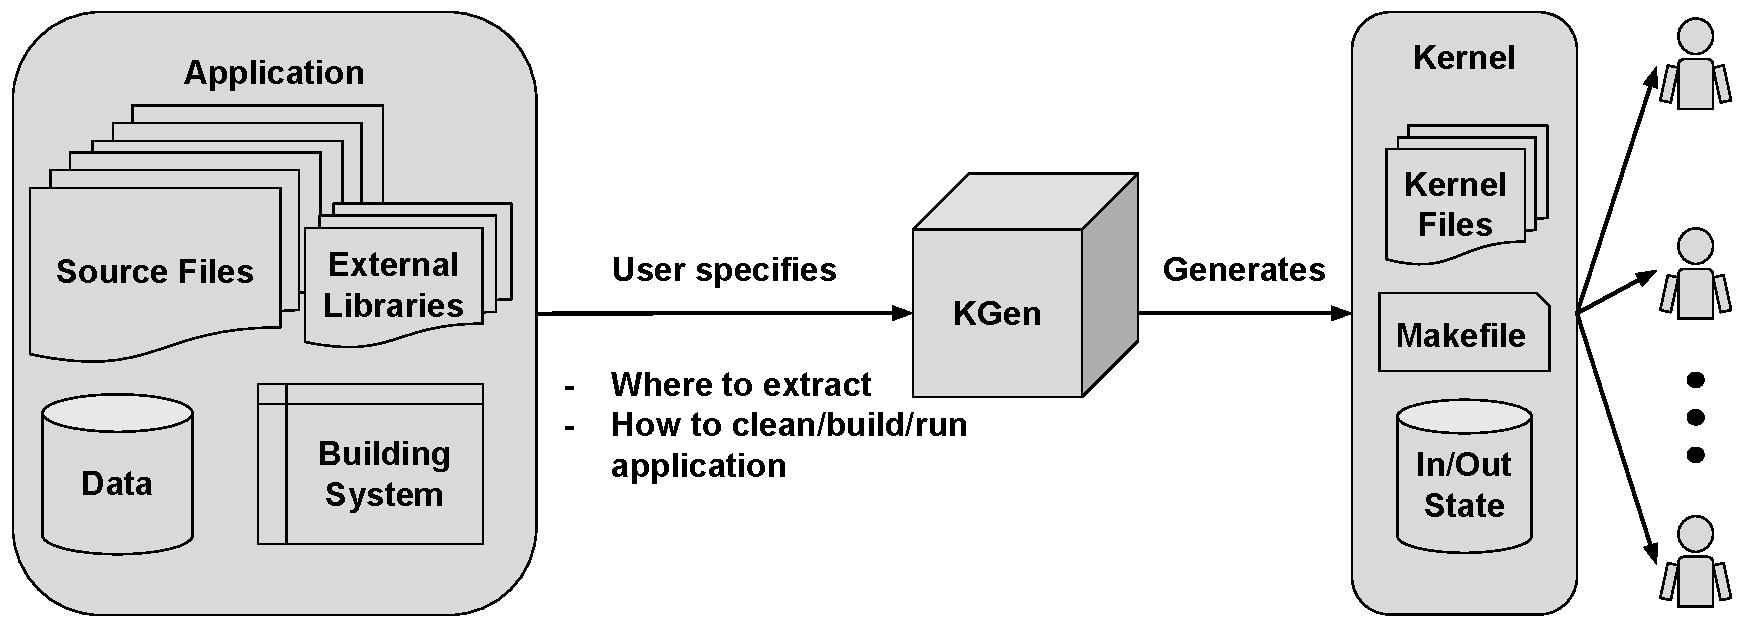
\includegraphics[width=12.0cm]{figures/kgen_workflow.pdf}
\end{center}
\caption{KGEN workflow.  {\color{red} Color not allowed in book, excessive space below image.}}
\label{fig:clmmem}
\end{figure}

Many scientific applications are large and complex. Depending on their configuration, it may takes more than an hour to complete compilation/execution. Instead, the size of generated kernel is generally between 1K to 100K source lines and it may take less than a minute to compile and run. Furthermore, a kernel does not have any dependencies to external library. Therefore, it could be easily built/run on multiple different machines. Once generated, kernel can be easily usable by collaborators.

Since a kernel is a just another software that can be compiled and run independently, its usage is not limited to a particular case. For example, There are several cases that KGen-generated kernel has been used successfully including:

Performance optimization: Several performance-critical parts of CESM were extracted using KGen and distributed to multiple performance engineers who independently optimized the generated kernels. Optimized kernels are collected and applied to CESM. Validating Float-point calculation among different platforms: The same CESM simulation on two different system showed different simulation result. A �suspicious� part of code was extracted using KGen. After large number of trial-and-errors on the kernel, it is found that the root cause was a FMA(Fused-Multiply-Add) instruction. Compiler bug report: A part of code having a compiler bug is extracted. A compiler bug is reported with the kernel so that the bug could be reproduced easily on compiler vendor site. Porting to GPU: A part of radiation physics code is extracted and shared with an external research team for porting it on GPU. Private benchmark for procurement: One of time consuming part of CESM is extracted and inserted in a benchmark suite for one of recent NCAR procurement.
A kernel generation example
KGen distribution contains several examples. This section briefly steps through one of the examples to show how to generate a kernel using KGen. First, please make sure that your system meets following prerequisites: Linux OS, Python (higher or equal to 2.7 but less than 3.0), Make build utility, Cpp C preprocessor and Strace system call tracer.

Downloading KGen: run following Git command on your local directory.
>>>  git clone  https://github.com/NCAR/KGen.git

Moving to an example directory: This example shows how to extract a region of Fortran code. Please read README to check if you need any modification for your system setting.
>>> cd ./KGen/example/simple-region

Extracting a kernel: run �make� in the example directory. The make command actually invokes KGen command shown below.
%>>>  $KGEN/bin/kgen src/update_mod.F90 --timing repeat=100 \ 
%  --cmd-clean "cd src; make clean" --cmd-build "cd src; make build" --cmd-run "cd src; make run" 
 
%The first argument specifies a path to a source file that contains KGen callsite directives. User can specify any executable region of Fortran code as a kernel region by wrapping the region with �begin_callsite� and �end_callsite� KGen directives. Next �--timing� option is to let KGen run a kernel region 100 times to increase accuracy of timing measurement. The last three options are to let KGen know how to clean/build/run the application. 

%Running a kernel: At this step, kernel files, state data files and Makefile are created in �kernel� subdirectory. Running KGen-generated Makefile in �kernel� directory will build/run the kernel and shows the results of verification and timing measurement of the kernel.
%>>> cd kernel; make


